\documentclass[11pt, a4paper]{article}

\usepackage[margin=2.2cm]{geometry}
\usepackage[T1]{fontenc}
\usepackage[utf8]{inputenc}
\usepackage{lmodern}
\usepackage{amsmath, amssymb, bm}
\usepackage{graphicx}
\usepackage{booktabs}
\usepackage{xcolor}
\usepackage{hyperref}
\usepackage{enumitem}
\usepackage{array}
\usepackage{longtable}
\usepackage{mdframed}
\usepackage{titlesec}
\usepackage{tikz}
\usetikzlibrary{positioning, shapes.geometric, arrows.meta, backgrounds, fit}
\usepackage{caption}
\usepackage{subcaption}
\usepackage{float}
\usepackage{parskip}

\hypersetup{colorlinks=true, linkcolor=blue!70!black, urlcolor=blue!70!black, citecolor=blue!70!black}

\definecolor{imperialblue}{RGB}{0,62,116}
\definecolor{lightblue}{RGB}{212,232,245}
\definecolor{lightyellow}{RGB}{255,252,220}
\definecolor{lightgreen}{RGB}{220,245,220}
\definecolor{lightred}{RGB}{255,230,225}
\definecolor{actionblue}{RGB}{225,240,255}

\titleformat{\section}{\large\bfseries\color{imperialblue}}{\thesection.}{0.5em}{}[\vspace{-2pt}\rule{\linewidth}{0.4pt}]
\titleformat{\subsection}{\normalsize\bfseries}{\thesubsection.}{0.5em}{}
\titleformat{\subsubsection}{\normalsize\itshape}{\thesubsubsection.}{0.5em}{}

%% Project macros
\newcommand{\bq}{\bm{q}}
\newcommand{\btau}{\bm{\tau}}
\newcommand{\bJ}{\bm{J}}
\newcommand{\bM}{\bm{M}}
\newcommand{\bC}{\bm{C}}
\newcommand{\bG}{\bm{G}}
\newcommand{\bPhi}{\bm{\Phi}}
\newcommand{\Ke}{K_{\mathrm{eff}}}
\newcommand{\Be}{B_{\mathrm{eff}}}
\newcommand{\dth}{\Delta\theta}

%% Coloured info boxes
\newmdenv[backgroundcolor=lightblue, linecolor=imperialblue!60,
          linewidth=1pt, innerleftmargin=8pt, innerrightmargin=8pt,
          innertopmargin=6pt, innerbottommargin=6pt, skipabove=6pt]{infobox}
\newmdenv[backgroundcolor=lightyellow, linecolor=orange!60,
          linewidth=1pt, innerleftmargin=8pt, innerrightmargin=8pt,
          innertopmargin=6pt, innerbottommargin=6pt, skipabove=6pt]{warnbox}
\newmdenv[backgroundcolor=lightgreen, linecolor=green!50!black,
          linewidth=1pt, innerleftmargin=8pt, innerrightmargin=8pt,
          innertopmargin=6pt, innerbottommargin=6pt, skipabove=6pt]{successbox}
\newmdenv[backgroundcolor=actionblue, linecolor=blue!50,
          linewidth=1pt, innerleftmargin=8pt, innerrightmargin=8pt,
          innertopmargin=6pt, innerbottommargin=6pt, skipabove=6pt]{actionbox}

% -------------------------------------------------------------------------
\title{\textbf{Meeting Notes: Progress Update 2 --- Exosuit-Assisted Control}\\[4pt]
       \large Cable-Driven Manipulator $+$ Series Elastic Exosuit $+$ Contraction Theory}
\author{Dipankar Bhattacharya (presenter) \\
        Thrishantha Nanayakkara (PI), Dagmar Sternad (collaborator), Salah Bazzi (collaborator)}
\date{20 May 2026}
% -------------------------------------------------------------------------

\begin{document}

\maketitle
\tableofcontents
\vspace{0.5cm}
\hrule
\vspace{0.4cm}

% =========================================================================
\section{Overview}
% =========================================================================

This document summarises the second progress meeting on the Exosuit Rehabilitation project.
Dipankar presented simulation and hardware progress covering: the dual-simulator platform
(PyDrake / Isaac~Sim), the 2-DOF cable-driven manipulator with series-elastic exosuit,
computed-torque control with exo co-contraction, disturbance attenuation results, online
parameter identification, and early contraction-theory (CCM) experiments.

\begin{infobox}
\textbf{Core research question:} Can a passively co-contracting exosuit at the elbow
(a) attenuate external disturbances, (b) make the dynamics simpler/more learnable for a
biological controller (brain), and (c) be formally certified via contraction theory?
\end{infobox}

% =========================================================================
\section{Simulation Platform}
% =========================================================================

\subsection{Dual-Simulator Design}

Two physics engines are maintained in parallel:

\begin{center}
\begin{tabular}{lll}
\toprule
\textbf{Simulator} & \textbf{Role} & \textbf{Strength} \\
\midrule
PyDrake + Meshcat & Analytical dynamics, LQR/CCM/CT design & Fast iteration, exact Jacobians \\
NVIDIA Isaac~Sim  & GPU-accelerated PhysX + Isaac Lab & RL/ML integration, sim-to-real \\
\bottomrule
\end{tabular}
\end{center}

The same Onshape CAD is used for both simulators and for the physical hardware, creating a
true \textbf{digital twin}.

\subsection{Model Pipeline}

\[
\text{Onshape (CAD)} \xrightarrow{\texttt{step1}} \text{URDF}
\xrightarrow{\texttt{step2}} \text{STL} \xrightarrow{\texttt{step3}} \text{OBJ}
\xrightarrow{} \text{PyDrake / Isaac Sim / Hardware}
\]

\begin{figure}[H]
\centering
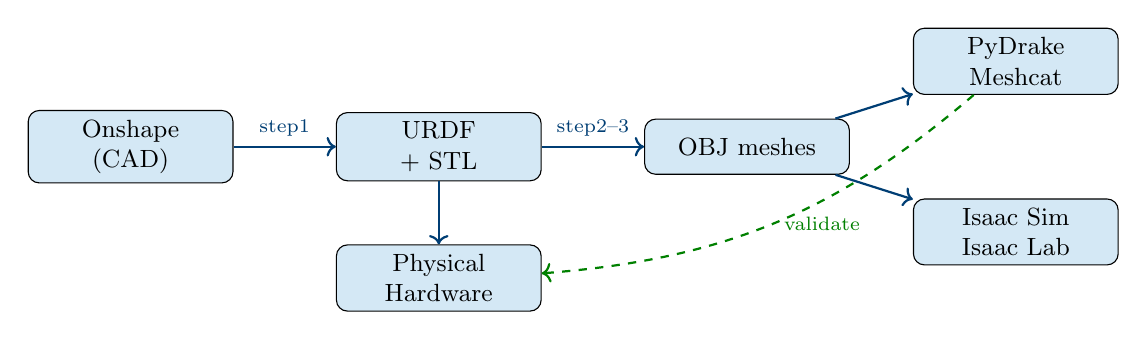
\begin{tikzpicture}[node distance=0.6cm and 1.3cm,
    box/.style={draw, rounded corners=4pt, minimum width=2.6cm, minimum height=0.7cm,
                fill=lightblue, align=center, font=\small},
    arr/.style={->, thick, color=imperialblue}]
  \node[box] (onshape) {Onshape\\(CAD)};
  \node[box, right=of onshape] (urdf) {URDF\\+ STL};
  \node[box, right=of urdf] (obj) {OBJ meshes};
  \node[box, above right=0.3cm and 0.8cm of obj] (drake) {PyDrake\\Meshcat};
  \node[box, below right=0.3cm and 0.8cm of obj] (isaac) {Isaac~Sim\\Isaac Lab};
  \node[box, below=0.8cm of urdf] (hw) {Physical\\Hardware};

  \draw[arr] (onshape) -- node[above,font=\scriptsize]{step1} (urdf);
  \draw[arr] (urdf) -- node[above,font=\scriptsize]{step2--3} (obj);
  \draw[arr] (obj) -- (drake);
  \draw[arr] (obj) -- (isaac);
  \draw[arr] (urdf) -- (hw);
  \draw[arr,dashed,color=green!50!black] (drake) to[bend left=18] node[right,font=\scriptsize]{validate} (hw);
\end{tikzpicture}
\caption{Simulation and hardware pipeline. The same URDF/OBJ assets feed both simulators and the physical device.}
\label{fig:pipeline}
\end{figure}

% =========================================================================
\section{Hardware Design}
% =========================================================================

\subsection{2-DOF Cable-Driven Manipulator}

\begin{center}
\begin{tabular}{lll}
\toprule
\textbf{Joint} & \textbf{Actuation} & \textbf{Motor} \\
\midrule
Shoulder (\texttt{link1\_base}) & Direct drive torque & AK60-6 (9\,Nm peak) \\
Elbow (\texttt{link2\_link1})   & Cable-driven via SEA & AK60-6 (9\,Nm peak) \\
\bottomrule
\end{tabular}
\end{center}

\textbf{Series Elastic Actuator (SEA) at elbow:}
\begin{itemize}[nosep]
  \item Motor wraps cables around a drive pulley ($r_p = 41$\,mm)
  \item Spring in series $\Rightarrow$ spring extension $\delta = r_p(\theta_m/N - q_2)$
  \item Spring force $F = k_s\,\delta + b_c\,\dot\delta$, joint torque $\tau_2 = r_p\,F$
  \item Encoders at both motor and joint allow real-time spring extension measurement
\end{itemize}

\subsection{Exosuit (Method B --- Antagonistic Co-contraction)}

\begin{itemize}[nosep]
  \item Two exo motors with cables routed over a centred elbow pulley ($r_{\mathrm{exo}} = 30$\,mm)
  \item Antagonistic arrangement: one cable tightens while the other goes slack
  \item Pre-tensioning both cables simultaneously $\Rightarrow$ \textbf{zero net torque}, but
        effective elbow stiffness increases:
\end{itemize}
\begin{equation}
  \Ke = 2\,k_{\mathrm{exo}}\,r_{\mathrm{exo}}^2
  \label{eq:keff}
\end{equation}

For $k_{\mathrm{exo}} = 8000$\,N/m and $r_{\mathrm{exo}} = 0.04775$\,m this gives
$\Ke = 36.48$\,Nm/rad.

\begin{infobox}
\textbf{Dagmar (meeting)}: ``An elegant way of manipulating a 2-joint arm with this cable
design. The added XO acting on the stiffness of the elbow --- that is \emph{new}.''

\textbf{Thrishantha}: ``I haven't seen that novel cable routing for a two-jointed arm before.''
\end{infobox}

% =========================================================================
\section{Control Architecture}
% =========================================================================

\begin{figure}[H]
\centering
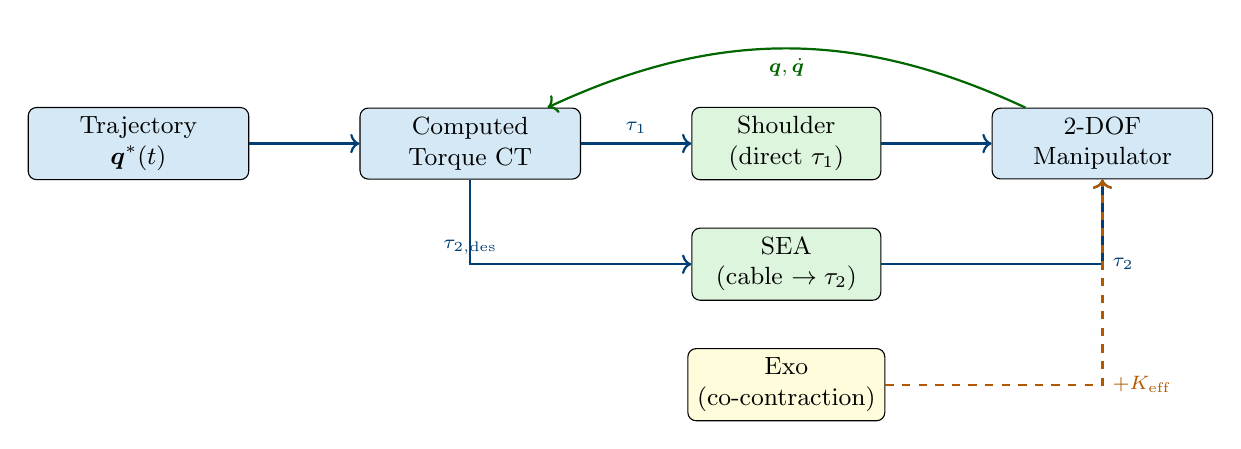
\begin{tikzpicture}[node distance=0.55cm and 1.5cm,
    box/.style={draw, rounded corners=3pt, minimum width=2.8cm, minimum height=0.65cm,
                fill=lightblue, align=center, font=\small},
    plant/.style={draw, rounded corners=3pt, minimum width=2.4cm, minimum height=0.65cm,
                fill=lightgreen, align=center, font=\small},
    exo/.style={draw, rounded corners=3pt, minimum width=2.4cm, minimum height=0.65cm,
                fill=lightyellow, align=center, font=\small},
    arr/.style={->, thick, color=imperialblue}]

  \node[box] (traj) {Trajectory\\$\bq^*(t)$};
  \node[box, right=1.4cm of traj] (ct) {Computed\\Torque CT};
  \node[plant, right=1.4cm of ct] (shoulder) {Shoulder\\(direct $\tau_1$)};
  \node[plant, below=0.6cm of shoulder] (sea) {SEA\\(cable $\to\tau_2$)};
  \node[exo, below=0.6cm of sea] (exo) {Exo\\(co-contraction)};
  \node[box, right=1.4cm of shoulder] (robot) {2-DOF\\Manipulator};

  \draw[arr] (traj) -- (ct);
  \draw[arr] (ct) -- node[above,font=\scriptsize]{$\tau_1$} (shoulder);
  \draw[arr] (ct) |- node[above,font=\scriptsize]{$\tau_{2,\mathrm{des}}$} (sea);
  \draw[arr] (shoulder) -- (robot);
  \draw[arr] (sea) -| node[right,font=\scriptsize]{$\tau_2$} (robot);
  \draw[arr,dashed,color=orange!70!black] (exo) -| node[right,font=\scriptsize]{$+\Ke$} (robot);

  \draw[arr, bend right=25, color=green!40!black] (robot) to
        node[below,font=\scriptsize]{$\bq,\dot\bq$} (ct);
\end{tikzpicture}
\caption{Layered control architecture. CT computes desired torques; SEA mediates the elbow
torque via cable/spring dynamics; the exo adds passive stiffness $\Ke$ when activated.}
\label{fig:arch}
\end{figure}

\subsection{Computed-Torque Controller}

\begin{align}
  \btau &= \bM(\bq)\,\ddot\bq_{\mathrm{des}} + \bC(\bq,\dot\bq)\,\dot\bq + \bG(\bq) \\
  \ddot\bq_{\mathrm{des}} &= \ddot\bq^* + K_d(\dot\bq^* - \dot\bq) + K_p(\bq^* - \bq)
  \label{eq:ct}
\end{align}

Parameters used in simulation: $K_p = 400$\,Nm/rad, $K_d = 80$\,Nm\,s/rad,
natural frequency $\omega_n = [20, 20]$\,rad/s, damping ratio $\zeta = [2,2]$.

\subsection{Exo Activation}

\begin{itemize}[nosep]
  \item \textbf{Transparent mode}: exo follows manipulator passively ($\tau_{\mathrm{exo}}\approx0$)
  \item \textbf{Co-contraction mode}: exo pre-tensioned by $\dth = 0.5$\,rad $\Rightarrow$
        passive restoring torque $\tau_{\mathrm{exo}} = -\Ke(q_2 - q_{2,\mathrm{anchor}})$
  \item Activation trigger: at $t = 4$\,s (or on disturbance detection)
\end{itemize}

% =========================================================================
\section{Simulation Results: Exo OFF vs.\ ON Under Disturbance}
% =========================================================================

\subsection{Experiment Setup}

\begin{center}
\begin{tabular}{ll}
\toprule
Parameter & Value \\
\midrule
Trajectory & Circle ($r = 40$\,mm, $v_{\max} = 80$\,mm/s) \\
Drive spring & $k_s = 200$\,N/m, $b_c = 8$\,N\,s/m \\
Disturbance & $\tau_{\mathrm{ext}} = 2.0\sin(2\pi \cdot 2\,\mathrm{Hz}\cdot t)$\,Nm, window $[8, 9.5]$\,s \\
Exo (ON case) & $k_{\mathrm{exo}} = 8000$\,N/m, $\dth = 0.5$\,rad, activate at $t=4$\,s \\
Motor & AK60-6 (9\,Nm limit), SEA torque mode \\
\bottomrule
\end{tabular}
\end{center}

\subsection{Manipulator Tracking Results}

\begin{figure}[H]
  \centering
  \begin{subfigure}[t]{0.48\textwidth}
    \includegraphics[width=\textwidth]{../../../plots/sea_exo_kexo8000_dth0.10_exo_off_20260520_132857_manip.png}
    \caption{Exo \textbf{OFF} (baseline). Large tracking error spikes during disturbance
             window ($t=8$--9.5\,s).}
    \label{fig:manip_off}
  \end{subfigure}\hfill
  \begin{subfigure}[t]{0.48\textwidth}
    \includegraphics[width=\textwidth]{../../../plots/sea_exo_kexo8000_dth0.50_exo_dist_sync_20260520_132422_manip.png}
    \caption{Exo \textbf{ON} ($\Ke = 36.48$\,Nm/rad). Disturbance spikes are significantly
             attenuated; drive motor works less.}
    \label{fig:manip_on}
  \end{subfigure}
  \caption{End-effector tracking error and joint torques: exo OFF vs.\ ON.
           Both plots use identical disturbance parameters.}
  \label{fig:manip_compare}
\end{figure}

\subsection{Exo Torque / Force Results}

\begin{figure}[H]
  \centering
  \begin{subfigure}[t]{0.48\textwidth}
    \includegraphics[width=\textwidth]{../../../plots/sea_exo_kexo8000_dth0.10_exo_off_20260520_132857_exo.png}
    \caption{Exo OFF: $\tau_{\mathrm{exo}} \approx 0$ (transparent mode).}
    \label{fig:exo_off}
  \end{subfigure}\hfill
  \begin{subfigure}[t]{0.48\textwidth}
    \includegraphics[width=\textwidth]{../../../plots/sea_exo_kexo8000_dth0.50_exo_dist_sync_20260520_132422_exo.png}
    \caption{Exo ON: passive exo applies $|\tau_{\mathrm{exo}}| \le 1.94$\,Nm
             --- the exo ``shares the load''.}
    \label{fig:exo_on}
  \end{subfigure}
  \caption{Exo cable force and torque signals. When ON, the exo provides passive
           antagonistic torque that reduces the drive motor's burden.}
  \label{fig:exo_compare}
\end{figure}

\begin{successbox}
\textbf{Logged metrics (exo ON, $\dth=0.5$\,rad):} \\
peak EE error = 11.98\,mm $|$ RMS EE error = 7.70\,mm $|$
peak $|q_2$ error$|$ = 4.61$^\circ$ $|$ RMS $q_2$ error = 2.87$^\circ$ $|$
peak $|\tau_{\mathrm{exo}}|$ = 1.94\,Nm $|$ peak $|\tau_{\mathrm{drive}}|$ = 1.39\,Nm
\end{successbox}

\begin{warnbox}
\textbf{Plot confusion (raised by Dagmar in meeting):} Both figures previously had identical
titles, making it unclear which was exo OFF and which was exo ON.
The larger torque in the exo-ON figure is $\tau_{\mathrm{exo}}$, \emph{not} the disturbance.
The disturbance amplitude is identical in both cases.
\textbf{Action:} Update figure titles to clearly distinguish
$\tau_{\mathrm{exo}}$, $\tau_{\mathrm{drive}}$, $\tau_{\mathrm{disturbance}}$.
\end{warnbox}

\subsection{PyDrake vs.\ Isaac Sim Comparison}

\begin{figure}[H]
  \centering
  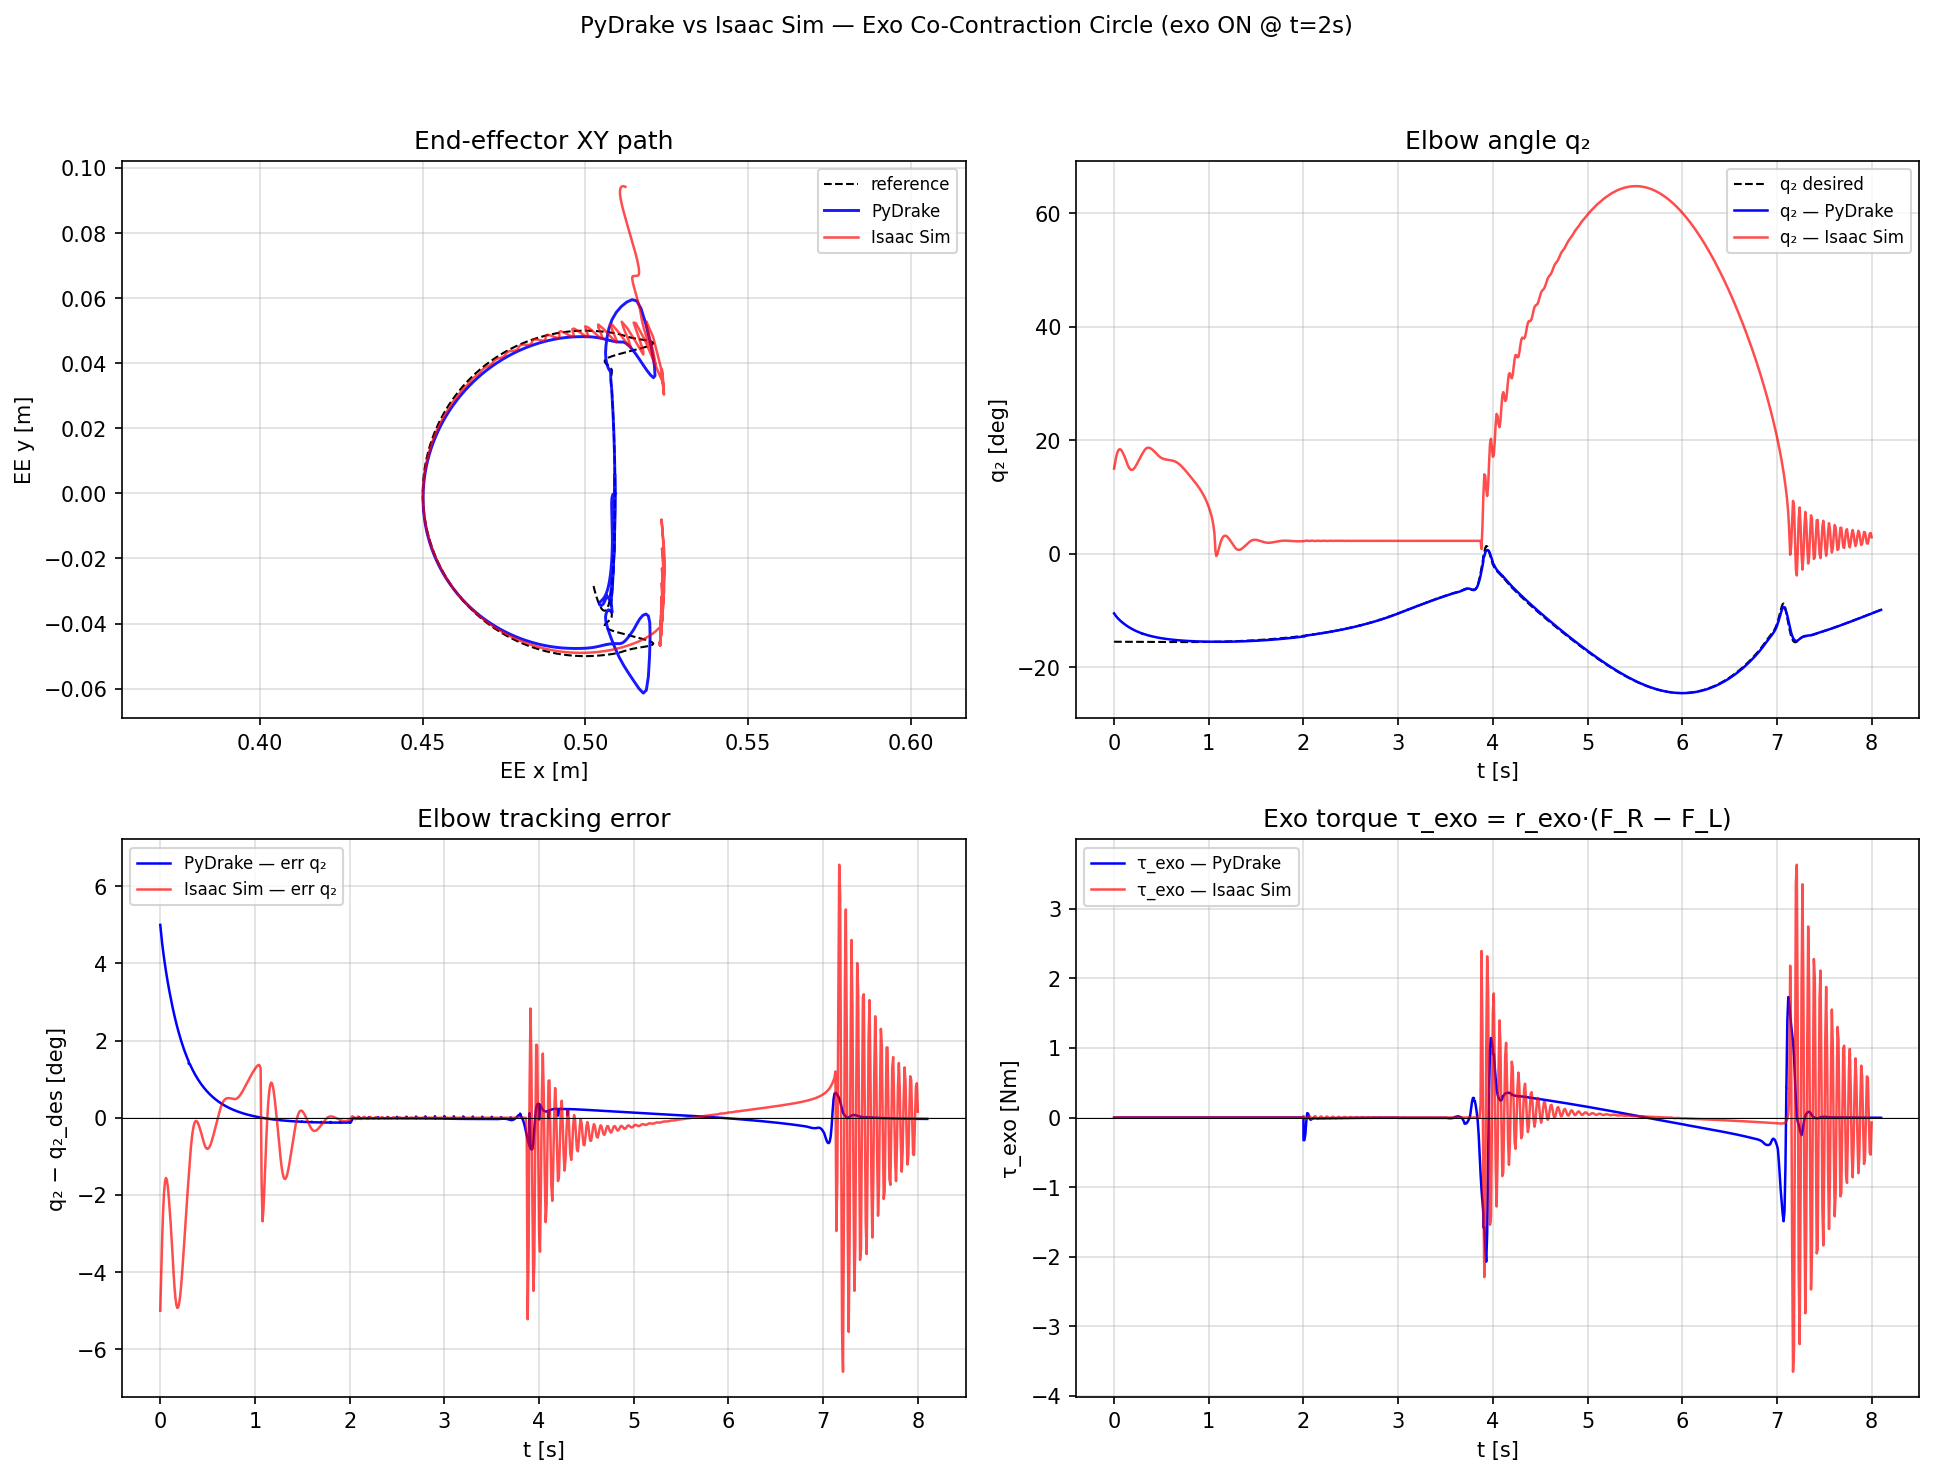
\includegraphics[width=0.8\textwidth]{../../../plots/exo_pydrake_vs_isaac_circle.png}
  \caption{Cross-validation: PyDrake (analytical) vs.\ Isaac Sim (PhysX) for a circle
           trajectory. Close agreement validates the digital twin.}
  \label{fig:pydrake_vs_isaac}
\end{figure}

% =========================================================================
\section{Parameter Learning: Probe $\to$ Identify $\to$ Adapt}
% =========================================================================

\subsection{Motivation}

In a rehabilitation context, the patient's elbow impedance $(\Ke, \Be)$ is unknown and
time-varying. The exosuit must identify these parameters and adapt the CT controller gains
so that the manipulator provides appropriate assistance.

\subsection{Algorithm}

\begin{enumerate}[nosep]
  \item \textbf{Probe}: inject a sinusoidal test torque into the elbow joint
  \item \textbf{Identify}: collect $(q_2, \dot q_2, \ddot q_2)$ samples; solve least-squares:
        \[
          \hat\theta = [\hat\Ke,\; \hat\Be]^\top = \arg\min_\theta
          \bigl\|\, \bPhi\,\theta - \btau_{\mathrm{elbow}} \bigr\|^2
        \]
        where $\bPhi = [q_2,\; \dot q_2]$ (regression matrix)
  \item \textbf{Adapt}: update CT gains using identified impedance; exo assists until
        the robot controller is accurate enough to fend off disturbances alone
\end{enumerate}

\begin{figure}[H]
  \centering
  \includegraphics[width=\textwidth]{../../../plots/learning_probe_20260520_153204.png}
  \caption{Probe-identify-adapt simulation. Top row: probe signal and elbow trajectory.
           Middle row: identified $\hat\Ke$ and $\hat\Be$ converging to ground truth
           ($\Ke = 36.48$\,Nm/rad). Bottom row: tracking error before/after adaptation.}
  \label{fig:learning}
\end{figure}

\begin{center}
\begin{tabular}{lll}
\toprule
Quantity & Ground truth & Identified \\
\midrule
$\Ke$ & 36.48\,Nm/rad & $\approx 45$\,Nm/rad (converging) \\
$\Be$ & --- & (pending) \\
\bottomrule
\end{tabular}
\end{center}

\subsection{Discussion: Limits of Linear Regression (meeting discussion)}

\begin{itemize}[nosep]
  \item \textbf{Salah}: ``How dependent is this on the trajectory type?
        Do you need a sinusoidal probe for a considerable time?''
        \\ $\to$ Currently only validated on one sinusoidal run. Generalisation is open.
  \item \textbf{Thrishantha}: ``Linear regression works for simple/linear oscillations.
        Complex non-sinusoidal trajectories may fail.''
  \item \textbf{Hypothesis}: The exo simplifies the dynamics enough that even simple
        linear regression can identify key impedance parameters.
        Without the exo, the dynamics are too noisy/nonlinear to identify.
\end{itemize}

\begin{infobox}
\textbf{Key hypothesis (Thrishantha):} ``The exo makes it a \emph{learnable} problem.
Without the exosuit, the brain doesn't see a pattern. So the existence of the exo just
makes it simple enough for the brain to learn. Can we test this experimentally?''
\end{infobox}

% =========================================================================
\section{Contraction Theory: CCM Analysis}
% =========================================================================

\subsection{Background}

Scripts \texttt{script\_11a} (YALMIP grid SDP) through \texttt{script\_14j} explore a
progression of contraction-theoretic controllers for the manipulator-exo system:

\begin{center}
{\small
\begin{tabular}{lll}
\toprule
\textbf{Script} & \textbf{Controller} & \textbf{Key finding} \\
\midrule
11a  & CCM (polynomial) vs LQR & LQR diverges at IC2; CCM global convergence \\
14a  & CT baseline (MATLAB)    & Reference for all comparisons \\
14b  & CCM constant metric $M=P$  & Exo adds $-\Ke$ term $\Rightarrow$ larger $\lambda$ \\
14e/f & CCM SDP, no-exo vs with-exo & SDP certifies $\lambda_{\max}(\text{exo}) > \lambda_{\max}(\text{no-exo})$ \\
14g  & Slotine original formulation & Side-by-side heatmaps \\
14h--j & C3M neural controller     & Learned certified controller; 10D augmented state \\
\bottomrule
\end{tabular}
}
\end{center}

\subsection{CCM Feasibility: No Exo vs.\ With Exo}

\begin{figure}[H]
  \centering
  \begin{subfigure}[t]{0.48\textwidth}
    \includegraphics[width=\textwidth]{../../../contraction-theory/script_14b_plot/14b_heatmap_sdp_exo0.png}
    \caption{CCM feasibility heatmap: \textbf{no exo}. Blue = contracting, Red = failing.
             Contraction only certified in a small region near origin.}
  \end{subfigure}\hfill
  \begin{subfigure}[t]{0.48\textwidth}
    \includegraphics[width=\textwidth]{../../../contraction-theory/script_14b_plot/14b_heatmap_sdp_exo1.png}
    \caption{CCM feasibility heatmap: \textbf{with exo}. Larger blue certified region ---
             the exo's $\Ke$ improves contraction rate $\lambda$.}
  \end{subfigure}
  \caption{YALMIP SDP feasibility: exo passive stiffness \emph{provably} increases the
           maximum contraction rate $\lambda_{\max}$ (scripts 14e/14f).}
  \label{fig:ccm_heatmap}
\end{figure}

\begin{figure}[H]
  \centering
  \includegraphics[width=0.75\textwidth]{../../../contraction-theory/script_14b_plot/14b_panels_circle.png}
  \caption{CCM constant-metric controller ($M{=}P$) tracking a circle trajectory with
           disturbance. Comparable to CT but with formal contraction guarantees.}
  \label{fig:ccm_tracking}
\end{figure}

\begin{figure}[H]
  \centering
  \includegraphics[width=0.75\textwidth]{../../../contraction-theory/script_14a_plot/14a_panels_circle.png}
  \caption{CT baseline (script 14a) --- same circle trajectory and disturbance conditions
           as Figure~\ref{fig:ccm_tracking}. Visual comparison: CCM
           (Fig.~\ref{fig:ccm_tracking}) achieves similar tracking with
           provably certified stability.}
  \label{fig:ct_tracking}
\end{figure}

\subsection{Why CCM? (Meeting Discussion)}

\begin{warnbox}
\textbf{Dipankar's gap}: ``I still couldn't really grasp how to use the CCM controller
for the manipulator-exo project. Why not just use CT? That's a question I still need to
think about.''
\end{warnbox}

\textbf{Salah's philosophical answer:}
\begin{quote}
``When you're interacting with an uncertain environment, you don't have an exact model of
all the types of disturbances that you'll encounter.
A Control Contraction Metric \emph{guarantees} that given some assumptions about the range
of $K$'s and $B$'s, these sets of gains are going to guarantee contraction / convergence /
attenuation, \emph{no matter what the disturbance magnitude}.''
\end{quote}

\textbf{Thrishantha's neuroscience parallel:}

The Purkinje cell / red nucleus system in the cerebellum uses climbing-fibre error signals
to update simple gains --- more like CCM (certified over a region) than full nonlinear
optimal control. The brain likely prefers a ``learnable'' representation that doesn't
require solving the full state-space problem.

% =========================================================================
\section{Research Gaps}
% =========================================================================

\begin{center}
{\small
\begin{tabular}{p{3.8cm}p{8.5cm}}
\toprule
\textbf{Gap} & \textbf{Description} \\
\midrule
CCM $\leftrightarrow$ exo connection &
  How to formally embed $\Ke(t)$ into CCM SDP.
  Scripts 14e/14f partially address this but not yet connected to the full system. \\[4pt]
Linear regression limits &
  Identification works for sinusoidal probe; fails for complex task dynamics
  with object loads or non-periodic motion. \\[4pt]
Human--robot gap &
  All work is simulation/robot-only. No human data yet. \\[4pt]
Plot clarity &
  $\tau_{\mathrm{exo}}$ vs $\tau_{\mathrm{drive}}$ vs $\tau_{\mathrm{disturbance}}$
  confusion in current figures. \\[4pt]
Sim-to-real &
  Controllers designed in simulation, not yet validated on assembled hardware. \\[4pt]
Learning generalisation &
  Parameters identified from sine probe may not transfer to
  circle/figure-8/task trajectories. \\[4pt]
CCM practical application &
  Bridge from toy polynomial system (script 11a) to
  full 6-DOF manipulator+exo with SEA dynamics. \\
\bottomrule
\end{tabular}
}
\end{center}

% =========================================================================
\section{Future Directions \& Paper Strategy}
% =========================================================================

\subsection{Stage 1 --- Hardware Completion (2--4 weeks)}
\begin{itemize}[nosep]
  \item Finish hardware assembly (placement student assisting)
  \item Calibrate AK60-6 motors and encoders on real device
  \item Implement CT + SEA + exo controllers on physical manipulator
  \item Verify sim $\leftrightarrow$ hardware consistency
\end{itemize}

\subsection{Stage 2 --- Robot-Only Experiments}
\begin{itemize}[nosep]
  \item Apply sinusoidal end-effector perturbations on hardware
  \item Record encoder data (exo OFF vs ON), compare to simulation metrics
  \item Use wireless EMG kit to measure muscle co-contraction as proxy for human response
\end{itemize}

\subsection{Stage 3 --- Human Experiments (ethics approval required)}
\begin{itemize}[nosep]
  \item Human holds end effector; robot applies sinusoidal perturbation
  \item Record reaching trajectory $+$ EMG $+$ exo ON/OFF conditions
  \item Elbow sling (ceiling mount) to isolate elbow dynamics (Thrishantha's paradigm)
  \item Compare human adaptation patterns to model predictions
\end{itemize}

\subsection{Paper Target}

\begin{infobox}
\textbf{Salah's suggestion:} ``The first thing we can publish is the mechanical design ---
a novel cable routing that emulates antagonistic muscles at the elbow.
This alone is publishable as a novel mechanism.''

\textbf{Dipankar's target:} TRO or IROS; contract ends October 2027.

\textbf{Dagmar:} ``The contraction theory part --- CCM --- maybe there is something
publishable there separately. In the meantime, collect human data because that is what
guides everything.''
\end{infobox}

% =========================================================================
\section{Decisions \& Action Items}
% =========================================================================

\subsection{Decisions Made}

\begin{center}
{\small
\begin{tabular}{ll}
\toprule
\textbf{Decision} & \textbf{Detail} \\
\midrule
Hardware first & Finish assembly before starting human experiments \\
EMG proxy & Use wireless EMG kit during robot perturbation to capture co-contraction \\
Ethics approval & Start application process for human study now \\
Fix plot labels & Distinguish $\tau_{\mathrm{exo}}$, $\tau_{\mathrm{drive}}$, $\tau_{\mathrm{disturbance}}$ in all figures \\
Learning study & Test identification with impulse probe, document regression limits \\
CCM integration & Deepen exo $\Ke$ embedding in SDP (scripts 14e/14f) \\
\bottomrule
\end{tabular}
}
\end{center}

\subsection{Action Items}

\begin{actionbox}
\begin{tabular}{lll}
\toprule
\textbf{Owner} & \textbf{Action} & \textbf{Priority} \\
\midrule
Dipankar & Finish hardware assembly + motor calibration & \textcolor{red}{\textbf{HIGH}} \\
Dipankar & Fix plot labels ($\tau_{\mathrm{exo}}$ vs $\tau_{\mathrm{disturbance}}$) & \textcolor{red}{\textbf{HIGH}} \\
Dipankar & Run impulse probe, document regression limits & MEDIUM \\
Dipankar & Connect CCM to manipulator+exo (scripts 14e/14f) & MEDIUM \\
Dipankar & Add $\hat\Ke$ vs ground truth comparison to learning plots & MEDIUM \\
Dipankar & Draft 1-page paper outline & MEDIUM \\
Thrishantha & Share sling/perturbation experimental paradigm reference & LOW \\
Team & Start ethics approval process for human study & LOW \\
\bottomrule
\end{tabular}
\end{actionbox}

% =========================================================================
\section{Open Questions for Next Meeting}
% =========================================================================

\begin{enumerate}
  \item \textbf{CCM synthesis}: Can $\Ke$ from the exo be embedded into the SDP LMI directly,
        and how much does it improve $\lambda_{\max}$?

  \item \textbf{Learning generalisation}: If we identify $\hat\Ke$ from a sinusoidal probe,
        does it transfer to a circle or figure-8 task with object loads?

  \item \textbf{Biological question}: Does the brain use something like CCM
        (certify over a set of disturbances) or something simpler
        (tune for a specific scenario)? How do we design an experiment to test this?

  \item \textbf{Paper scope}: Mechanism-only first paper, or include
        simulation + CCM analysis together?

  \item \textbf{Human protocol}: End-effector hold + sinusoidal perturbation vs.\ elbow
        sling + perturbation --- which is simpler for ethics approval and most informative?
\end{enumerate}

% =========================================================================
\section*{Notable Quotes}
% =========================================================================

\begin{mdframed}[backgroundcolor=gray!8, linecolor=gray!50]
\textit{``Our hypothesis is the brain will learn better with the exosuit. Without the exosuit
it's very random and the brain doesn't see a pattern. The exo makes it a learnable problem.''}
\hfill --- Thrishantha
\end{mdframed}

\vspace{4pt}
\begin{mdframed}[backgroundcolor=gray!8, linecolor=gray!50]
\textit{``A Control Contraction Metric guarantees that these K's and B's are going to
guarantee contraction, no matter what the disturbance magnitude. That's my philosophical
answer to the `why CCM'.''} \hfill --- Salah
\end{mdframed}

\vspace{4pt}
\begin{mdframed}[backgroundcolor=gray!8, linecolor=gray!50]
\textit{``That is new, right? An elegant way of manipulating a two-joint arm with this cable
design. The added XO acting on the stiffness of the elbow --- that is new.''}
\hfill --- Dagmar
\end{mdframed}

\vspace{4pt}
\begin{mdframed}[backgroundcolor=gray!8, linecolor=gray!50]
\textit{``It actually opened a lot of questions. I'll think about all of them.
Hopefully we can do something very soon.''}
\hfill --- Dipankar
\end{mdframed}

\vspace{1cm}
\hrule
\vspace{4pt}
{\small\textit{Notes compiled from transcript:
\texttt{transcripts/2026\_05\_20\_Progress Update 2\_ Exosuit .vtt}.
Figures from \texttt{plots/} and \texttt{contraction-theory/script\_14*/}.}}

\end{document}
